\documentclass{beamer}
\usepackage{amsthm}
\usepackage{amsmath}
\usepackage{amssymb}
\usepackage{graphicx}
\usepackage[utf8]{inputenc}
\usepackage[slovene]{babel}
\usepackage{graphicx}
\usepackage{amsbsy}
\usepackage{sidecap}
\usetheme{Madrid}
\theoremstyle{definition} 
\newtheorem{definicija}{Definicija}[section]
\newtheorem{primer}[definicija]{Primer}


\renewcommand\endprimer{\hfill$\diamondsuit$}


\theoremstyle{plain}
\newtheorem{lema}[definicija]{Lema}
\newtheorem{izrek}[definicija]{Izrek}
\newtheorem{trditev}[definicija]{Trditev}
\newtheorem{posledica}[definicija]{Posledica}
\newtheorem{zgled}[definicija]{Zgled}
\usecolortheme{beaver}
\title[Iterativni izračun Nashevega ravnovesja]{Iterativni izračun Nashevega ravnovesja v matričnih igrah}
\author[Eva Babnik]{Eva Babnik \\ Mentor: prof. dr. Sergio Cabello Justo}
\institute[]{Fakulteta za matematiko in fiziko}
\date{2. junij 2022}
\begin{document}
\frame{\titlepage}
\begin{frame}
\frametitle{Cilji naloge in uporabljeno programsko okolje}

\begin{itemize}
\item Implementacija dveh iterativnih metod, ki vrneta vrednost igre in optimalno strategijo v matričnih igrah z ničelno vsoto za dva igralca.
\item Analiza konvergence implementiranih metod.
\item Preprosta aplikacija, ki iterativno izračuna rešitev igre.
\item  \textit{Python}, programski jezik \textit{R}.
\end{itemize}

\end{frame}
\begin{frame}
    \frametitle{Problem}
    \begin{itemize}
        \item Matrika izplačil $ (a_{i,j}), \; i = 1, \cdots, m, \; \;   j =1,\cdots,n.$
        \item 1.igralec izbere eno izmed $m$ vrstic z verjetnostjo $x_i$, 2. igralec pa enega izmed $n$ stolpcev z verjetnostjo $y_j$.
        \item Veljati mora:
        \begin{equation}
            \label{eqn:e1}
            x_i \geq 0,
        \end{equation}
        \begin{equation}
            \label{eqn:e2}
            \sum x_i = 1,
        \end{equation}
        \begin{equation}
            \label{eqn:e3}
        y_i \geq 0,
        \end{equation}
        \begin{equation}
            \label{eqn:e4}
            \sum y_i = 1.
        \end{equation}
        \item Vrednost igre je definirana kot

        \begin{equation*}
            v = \min_j \sum_{i} a_{ij}x_i = \max_i \sum_j a_{ij} y_j,
        \end{equation*}
        pri čemer ($x, y$), ki rešita zgornjo enakost predstavljata rešitev igre.
    \end{itemize}
\end{frame}

\begin{frame}
    \frametitle{Metoda I}

    Definirajmo:
    \begin{equation*}
        \begin{split}
        A_i = [a_{1i}, \cdots, a_{mi}, \underbrace{0, \cdots, 0}_{n - \text{komponent}}, -1], \\
        A_{0i} = [\underbrace{1, \cdots, 1}_{m-\text{komponent}}, \underbrace{0, \cdots, 0}_{n-\text{komponent}}, 0] \\
        \text{za} \, \, i = 1, \cdots, n
        \end{split}
    \end{equation*} 
    in 
    \begin{equation*}
        \begin{split}
        A_i = [\underbrace{0, \cdots, 0}_{m - \text{komponent}},-a_{i-n, 1}, \cdots, -a_{i - n, n}, 1], \\
         A_{0i} = [\underbrace{0, \cdots, 0}_{m-\text{komponent}},\underbrace{1, \cdots, 1}_{n-\text{komponent}},  0] \\
        \text{za} \, \, i = n + 1, \cdots, m + n.
        \end{split}
    \end{equation*} 
    \end{frame}
    \begin{frame}
        \frametitle{Metoda I}
    
    Definirajmo še rešitev igre $z^* = [x^*, y^*, v^*]$, ki mora poleg prej naštetih pogojev, ustrezati še:

    \begin{equation}
        \label{eqn:e5}
    A_i \cdot z^* \geq 0 \, \, \text{za} \, \, i = 1, \cdots, m + n.
    \end{equation}
\end{frame}

\begin{frame}
    \frametitle{Metoda I}
    \begin{itemize}
        \item Izberemo poljuben začetni vektor $z^{(1)}$, ki zadošča \ref{eqn:e1}, \ref{eqn:e2}, \ref{eqn:e3}, \ref{eqn:e4} in \ref{eqn:e5} . 
        \item Predpostavimo, da smo prišli na $k$-ti korak in dobili vektor $z^{(k)}$,  ki ustreza \ref{eqn:e1}, \ref{eqn:e2}, \ref{eqn:e3} in \ref{eqn:e4}. Če velja tudi
    \ref{eqn:e5}, je $z^{(k)}$ rešitev igre in smo zaključili. Sicer pa:
    \begin{itemize}
     \item Najdemo tak $j_k$, da velja $A_{j_k} \cdot z^{(k)} \leq A_i \cdot z^{(k)}$ $\; \forall \; $ $i = 1, \cdots, m + n$. 
     \item $\bar{z}^{(k+1)} = z^{(k)} + \alpha B_{j_k} + \beta B_{0j_k}$,
    kjer je
    \begin{equation*}
        \alpha = - z^{(k)} \cdot B_{j_k} [1 - \cos^2{\theta_{j_k}}]^{-1},
    \end{equation*}
    \begin{equation*}
        \beta = b_{0j_k} - [z^{(k)} + \alpha B_{j_k}] \cdot B_{0j_k},
    \end{equation*}
    \begin{equation*}
        b_{0j_k} = \frac{1}{(A_{0j_k}\cdot A_{0j_k})^{1/2}},
    \end{equation*}
    \begin{equation*}
    B_{j_k} = \frac{A_{j_k}}{(A_{j_k} \cdot A_{j_k})^{1/2}}, 
    \end{equation*}
    \begin{equation*}
    B_{0j_k} = \frac{A_{0j_k}}{(A_{0j_k}\cdot A_{0j_k})^{1/2}}
    \end{equation*}
    in 
    \begin{equation*}
     \cos{\theta_{j_k}} = \frac{A_{0j_k} \cdot A_{j_k}}{(A_{0j_k}\cdot A_{0j_k})^{1/2}(A_{j_k}\cdot A_{j_k})^{1/2}}.
    \end{equation*}
\end{itemize}
\end{itemize}
\end{frame}
\begin{frame}
\frametitle{Metoda I}
     \begin{itemize}
        \item Predpostavimo, da velja  $j_k < (n +1)$.
        \item Če $A_i \cdot z^* \geq 0 \, \, \forall i = 1: \, (m+n)$:
        \begin{itemize}
            \item $z^{k+1} = \bar{z}^{k+1}$
        \end{itemize}
        \item Sicer:
        \begin{itemize}
           \item Vse negativne $x$-komponente vektorja $\bar{z}^{k+1}$ nastavimo na 0.
           \item Izračunamo vsote  $\bar{x}_i^{(k+1)} + \frac{\sum_{i=1}^r \bar{x}_i^{(k+1)}}{m - r} $ za $i = r +1, \cdots, m$, kjer 
           so $\bar{x}_1^{(k+1)}, \cdots, \bar{x}_r^{(k+1)}, \, \, r < m$ negativne komponente vektorja $\bar{z}^{(k+1)}$.
           \item Za vsak tak $i$, za katerega
           je vsota negativna: $x_i^{(k+1)} = 0$.
           \item Če nobena vsota ni negativna, lahko tvorimo preostanek vektorja $z^{(k+1)}$.
           \item Če so nekatere vsote za $i = r+1, \cdots, r +s$ negativne, ponovno izračunamo vsote 
           $\bar{x}_i^{(k+1)} + \frac{\sum_{i=1}^{r+s} \bar{x}_i^{(k+1)}}{m - (r+s)} $ za $i = r + s, \cdots, m$ in postopek ponavljamo, dokler nobena od vsot ni nenegativna.
        \end{itemize}
    \end{itemize}
\end{frame}
\begin{frame}
\frametitle{Metoda I}
    \begin{itemize}
        \item Predpostavimo, da za $i = 1, \cdots, t$ velja, da je $\bar{x}_i^{(k+1)} \leq 0$ ali pa, da je $\bar{x}_i^{(k+1)}$ tak, da je zanj katera od zgoraj definiranih vsot negativna. 
        \item Tvorimo preostanek vektorja $z^{(k+1)}$:

    \begin{equation*}
        x_1^{(k+1)} = \cdots = x_t^{(k+1)} = 0,
    \end{equation*}  
    \begin{equation*}
        x_i^{(k+1)} = \bar{x}^{(k+1)} +  \frac{\sum_{i=1}^{t}\bar{x}_i^{(k+1)}}{m-t} \, \, \text{za} \, \, i = t+1, \cdots, m,
    \end{equation*}
    \begin{equation*}
        y_j^{(k+1)} = \bar{y}_j^{(k+1)} \, \, \text{za} \, \, j = 1, \cdots, n,
    \end{equation*}
    \begin{equation*}
        v^{(k+1)} = \bar{v}^{(k+1)}.
    \end{equation*}
    
\end{itemize}
\end{frame}
\begin{frame}
    \frametitle{Metoda II}
    \begin{itemize}
    \item 1. igralec igra poljubno čisto strategijo $x_{i_1}$.
    \item Definiramo vektor akumulativnih vsot $A^{(1)} = [a_1^{(1)}, \cdots, a_n^{(1)}]$ \, ($A^{(1)}$ = $i_1$-ta vrstica $A$). 
    \item 2. igralec igra čisto strategijo $y_{j_1}$ (za $j_1$  velja: $a_{j_1}^{(1)}$ = $\min \{a_1^{(1)}, \cdots, a_n^{(1)}\}$).
    \item Definiramo vektor akumulativnih vsot $B^{(1)} = [b_1^{(1)}, \cdots, b_m^{(1)}]$, \, ($B^{(1)}= j$-ti stolpec matrike).
    \item 1. igralec igra čisto strategijo $x_{i_2}$ (za $i_2$ velja: $b_{j_2}^{(1)} = max\{b_1^{(1)}, \cdots, b_m^{(1)}\}$).
    \item 1. igralec vektorju $A^{(1)}$ prišteje $i_2$ - to vrstico matrike, zatem pa 2. igralec igra na enak način kot prej.
    \item Postopek ponavljamo.
    \end{itemize}
\end{frame}
\begin{frame}
    \frametitle{Metoda II}
    Zaporedji  $\frac{\sum_{n=1}^k x_{i_n}}{k}$, $\,\frac{\sum_{n=1}^k y_{i_n}}{k}$  ali konvergirata k optimalni strategiji $x^*, y^*$. \\
     $v_1 = \max_{k = 1, 2, \cdots} \frac{\min_{i \in (1, \cdots, n)} a_i^{(k)}}{k}$, \\
$v_2 = \min_{k = 1, 2, \cdots} \frac{\max_{i \in (1, \cdots, m)} b_i^{(k)}}{k}$.
\end{frame}
\begin{frame}
\frametitle{Analiza konvergence, časovna zahtevnost in rezultati}
\begin{itemize}
\item Časovna zahtevnost prvega algoritma: $\mathcal{O}(k (m^2 \vee n^2))$.
\item Časovna zahtevnost drugega algoritma: $\mathcal{O}(k)$.
\item Meritve opravljene s prenosnim računalnikom s procesorjem 2.40GHz Intel(R) Core(TM) i5-6300U CPU in 8GB spomina. 
\item Število ponovitev poskusov: 10.
\end{itemize}
\end{frame}

\begin{frame}
    \frametitle{Analiza konvergence in časovne zahtevnosti za prvo igro}
    \begin{equation*}
        \begin{bmatrix}
            4 & 3\\
            2 & 4\\
            5 & 2
        \end{bmatrix}
        \end{equation*}
     $v^* = \frac{10}{3}$, \\
     $x^* = [\frac{2}{3}$, \\
     $\frac{1}{3}, 0]$, $y^* = [\frac{1}{3}, \frac{2}{3}]$.
\end{frame}
\begin{frame}
    \frametitle{Vrednost prve igre v odvisnosti od števila iteracij}
    \begin{figure}
        \centering
        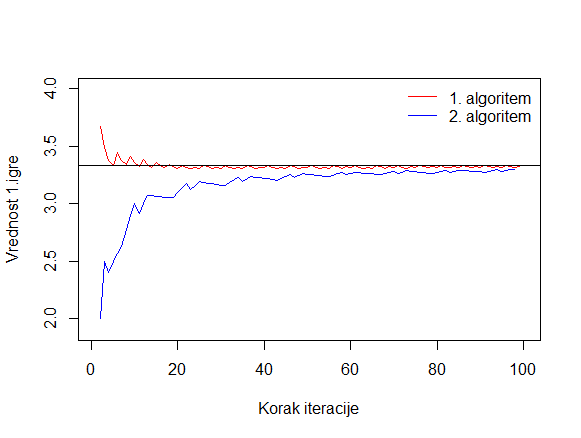
\includegraphics[width=12cm]{1.igra_vred.png}
        \caption{Vrednosti prve matrične igre}
        \label{fig:vred1}
      \end{figure}
\end{frame}
\begin{frame}
    \frametitle{Napaka algoritmov $||z^* - z^{k}||_{\infty}$ za prvo matrično igro}
    \begin{figure}
        \centering
        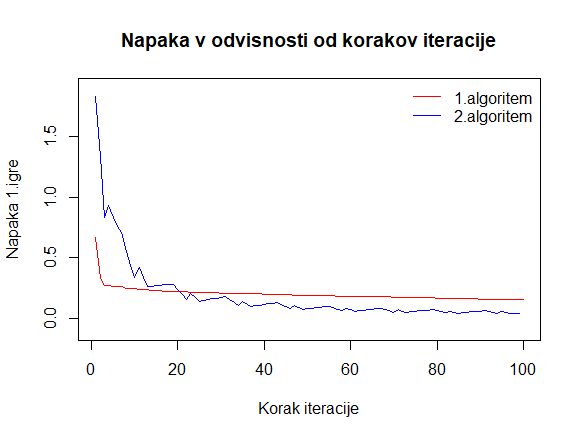
\includegraphics[width=12cm]{napaka1.png}
        \caption{Napaka algoritmov za prvo matrično igro}
        \label{fig:napaka1}
      \end{figure}
\end{frame}
\begin{frame}
    \frametitle{Analiza konvergence in časovne zahtevnosti za prvo igro}
    \begin{table}[]
        \resizebox{9cm}{!}{\begin{tabular}{c|llll|llll|}
        \cline{2-9}
                                                                                                     & \multicolumn{4}{c|}{1. metoda}                                                                                                                       & \multicolumn{4}{c|}{2. metoda}                                                                                                                                                                                    \\ \cline{2-9} 
                                        & \multicolumn{1}{l|}{čas}    & \multicolumn{1}{l|}{v}       & \multicolumn{1}{l|}{x}                                                                   & y                                                         & \multicolumn{1}{l|}{čas}    & \multicolumn{1}{l|}{v}       & \multicolumn{1}{l|}{x}                                                                   & y                                                         \\ \hline
        \multicolumn{1}{|c|}{k =  1}    & \multicolumn{1}{l|}{0.0020} & \multicolumn{1}{l|}{3}       & \multicolumn{1}{l|}{\begin{tabular}[c]{@{}l@{}}0.33333\\ 0.33333\\ 0.33333\end{tabular}} & \begin{tabular}[c]{@{}l@{}}0\\ 1\end{tabular}             & \multicolumn{1}{l|}{0.0009} & \multicolumn{1}{l|}{1.5}  & \multicolumn{1}{l|}{\begin{tabular}[c]{@{}l@{}}0.5\\ 0.5\\ 0\end{tabular}}               & \begin{tabular}[c]{@{}l@{}}0\\ 0.5\end{tabular}           \\ \hline
        \multicolumn{1}{|c|}{k = 2}     & \multicolumn{1}{l|}{0.0020} & \multicolumn{1}{l|}{3.49020} & \multicolumn{1}{l|}{\begin{tabular}[c]{@{}l@{}}0.33333\\ 0.33333\\ 0.33333\end{tabular}} & \begin{tabular}[c]{@{}l@{}}0.5\\ 0.5\end{tabular}         & \multicolumn{1}{l|}{0.0014} & \multicolumn{1}{l|}{2}  & \multicolumn{1}{l|}{\begin{tabular}[c]{@{}l@{}}0.66667\\ 0.33333\\ 0\end{tabular}}       & \begin{tabular}[c]{@{}l@{}}0.33333\\ 0.33333\end{tabular} \\ \hline
        \multicolumn{1}{|c|}{k = 10}    & \multicolumn{1}{l|}{0.0155} & \multicolumn{1}{l|}{3.31150} & \multicolumn{1}{l|}{\begin{tabular}[c]{@{}l@{}}0.34199\\ 0.45804\\ 0.19997\end{tabular}} & \begin{tabular}[c]{@{}l@{}}0.34425\\ 0.65575\end{tabular} & \multicolumn{1}{l|}{0.0020} & \multicolumn{1}{l|}{3}  & \multicolumn{1}{l|}{\begin{tabular}[c]{@{}l@{}}0.45454\\ 0.45454\\ 0\end{tabular}}       & \begin{tabular}[c]{@{}l@{}}0.27273\\ 0.63636\end{tabular} \\ \hline
        \multicolumn{1}{|c|}{k = 50}    & \multicolumn{1}{l|}{0.0156} & \multicolumn{1}{l|}{3.33100} & \multicolumn{1}{l|}{\begin{tabular}[c]{@{}l@{}}0.47646\\ 0.40436\\ 0.11918\end{tabular}} & \begin{tabular}[c]{@{}l@{}}0.33100\\ 0.66900\end{tabular} & \multicolumn{1}{l|}{0.0030} & \multicolumn{1}{l|}{3.25490}  & \multicolumn{1}{l|}{\begin{tabular}[c]{@{}l@{}}0.64706\\ 0.33333\\ 0.01961\end{tabular}} & \begin{tabular}[c]{@{}l@{}}0.35294\\ 0.62746\end{tabular} \\ \hline
        \multicolumn{1}{|c|}{k = 100}   & \multicolumn{1}{l|}{0.0369} & \multicolumn{1}{l|}{3.33147} & \multicolumn{1}{l|}{\begin{tabular}[c]{@{}l@{}}0.51447\\ 0.39017\\ 0.09536\end{tabular}} & \begin{tabular}[c]{@{}l@{}}0.33146\\ 0.66854\end{tabular} & \multicolumn{1}{l|}{0.0049} & \multicolumn{1}{l|}{3.28713}  & \multicolumn{1}{l|}{\begin{tabular}[c]{@{}l@{}}0.66337\\ 0.32673\\ 0.00990\end{tabular}} & \begin{tabular}[c]{@{}l@{}}0.33663\\ 0.65347\end{tabular} \\ \hline
        \multicolumn{1}{|c|}{k = 500}   & \multicolumn{1}{l|}{0.0953} & \multicolumn{1}{l|}{3.33301} & \multicolumn{1}{l|}{\begin{tabular}[c]{@{}l@{}}0.64108\\ 0.34289\\ 0.01603\end{tabular}} & \begin{tabular}[c]{@{}l@{}}0.33302\\ 0.66670\end{tabular} & \multicolumn{1}{l|}{0.0156} & \multicolumn{1}{l|}{3.32335} & \multicolumn{1}{l|}{\begin{tabular}[c]{@{}l@{}}0.66467\\ 0.33333\\ 0.00200\end{tabular}} & \begin{tabular}[c]{@{}l@{}}0.33134\\ 0.66667\end{tabular} \\ \hline
        \multicolumn{1}{|c|}{k = 1000}  & \multicolumn{1}{l|}{0.1207} & \multicolumn{1}{l|}{3.33330} & \multicolumn{1}{l|}{\begin{tabular}[c]{@{}l@{}}0.66391\\ 0.33436\\ 0.00173\end{tabular}} & \begin{tabular}[c]{@{}l@{}}0.33330\\ 0.66670\end{tabular} & \multicolumn{1}{l|}{0.0312} & \multicolumn{1}{l|}{3.33290} & \multicolumn{1}{l|}{\begin{tabular}[c]{@{}l@{}}0.66633\\ 0.33257\\ 0.00010\end{tabular}} & \begin{tabular}[c]{@{}l@{}}0.33367\\ 0.66533\end{tabular} \\ \hline
        \multicolumn{1}{|c|}{k = 15000} & \multicolumn{1}{l|}{2.4360} & \multicolumn{1}{l|}{3.33333} & \multicolumn{1}{l|}{\begin{tabular}[c]{@{}l@{}}0.66667\\ 0.33333\\ 0\end{tabular}}       & \begin{tabular}[c]{@{}l@{}}0.33333\\ 0.66667\end{tabular} & \multicolumn{1}{l|}{0.4397} & \multicolumn{1}{l|}{3.33304} & \multicolumn{1}{l|}{\begin{tabular}[c]{@{}l@{}}0.66656\\ 0.33338\\ 0.00007\end{tabular}} & \begin{tabular}[c]{@{}l@{}}0.33338\\ 0.66656\end{tabular} \\ \hline
        \end{tabular}}
        \caption{Primerjava rezultatov za 1. igro}
        \label{table:1igra}
        \end{table} 
\end{frame}
\begin{frame}
    \frametitle{Analiza konvergence in časovne zahtevnosti za drugo igro}
    \begin{equation*}
        \begin{bmatrix}
            0 & -1 & -2 & 0 & 0 & 2 & 1\\
            1 & 0 & 0 & 4  & 0 & 0 & -1\\
            2 & 0 & 0 & -1 & 1 & 0 & -1\\
            0 &-4 & 1 & 0 & 0 & -1 & 1\\
            0 & 0 & -1 & 0 & 0 & -3 & 1\\
            -2 & 0 & 0 & 1 & 3 & 0 & -1\\
            -1 & 1 & 1 & -1 & -1 & 1 & 0 
        \end{bmatrix}
        \end{equation*}
        
        $v^* = 0,$ \\
        $x^* = [1/9, 1/9, 15/90, 5/90, 15/90, 5 / 90, 1 /3]$, \\
        $y^* = [1 / 9, 1 / 9, 15/90, 5 / 90, 15 / 90,  5 / 90, 1 /3]$. 
\end{frame}
\begin{frame}
    \frametitle{Vrednost druge igre v odvisnosti od števila iteracij}
    \begin{figure}
        \centering
        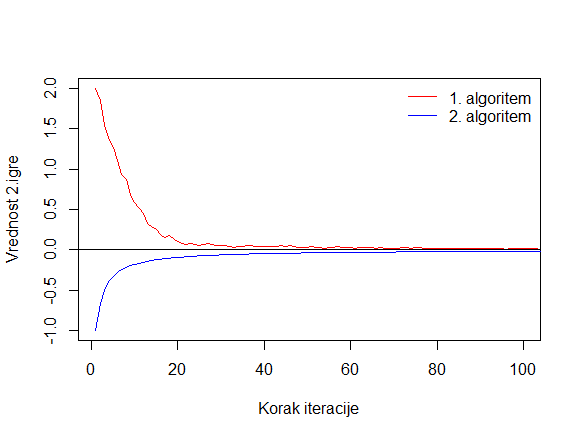
\includegraphics[width=10cm]{2igra_vrednosti.png}
        \caption{Vrednosti druge matrične igre}
        \label{fig:vred2}
      \end{figure}
    \end{frame}
\begin{frame}
    \frametitle{Napaka algoritmov $||z^* - z^{k}||_{\infty}$ za prvo matrično igro}
    \begin{figure}
        \centering
        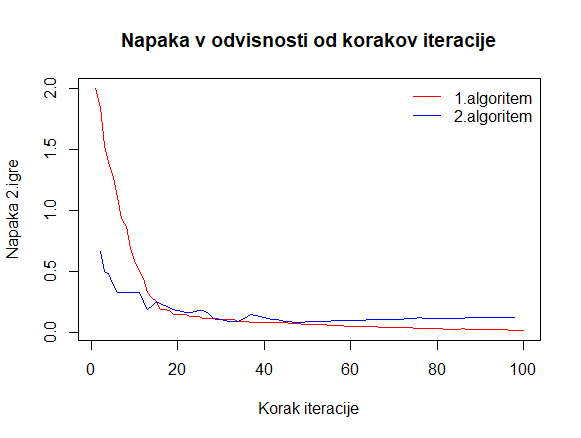
\includegraphics[width=12cm]{napaka2igra.png}
        \caption{Napaka algoritmov za drugo matrično igro}
        \label{fig:napaka2}
      \end{figure}
\end{frame}
\begin{frame}
    \frametitle{Analiza konvergence in časovne zahtevnosti za drugo igro}
    \begin{table}[]
        \resizebox{4.6cm}{!}{\begin{tabular}{c|llll|llll|}
        \cline{2-9}
                                        & \multicolumn{4}{c|}{1. metoda}                                                                                                                                                                                                                                                                                        & \multicolumn{4}{c|}{2. metoda}                                                                                                                                                                                                                                                                                  \\ \cline{2-9} 
                                        & \multicolumn{1}{l|}{čas}     & \multicolumn{1}{l|}{v}       & \multicolumn{1}{l|}{x}                                                                                                                  & y                                                                                                             & \multicolumn{1}{l|}{čas}     & \multicolumn{1}{l|}{v}       & \multicolumn{1}{l|}{x}                                                                                                             & y                                                                                                            \\ \hline
        \multicolumn{1}{|c|}{k =  1}    & \multicolumn{1}{l|}{0.00365} & \multicolumn{1}{l|}{1.84615} & \multicolumn{1}{l|}{\begin{tabular}[c]{@{}l@{}}0.01282\\ 0.16667\\ 0.16667\\ 0\\ 0.16667\\ 0.16667\\ 0.32051\end{tabular}}              & \begin{tabular}[c]{@{}l@{}}0.14286\\ 0.14286\\ 0.14286\\ 0.14286\\ 0.14286\\ 0.14286\\ 0.14286\end{tabular}   & \multicolumn{1}{l|}{0.00165} & \multicolumn{1}{l|}{-1}    & \multicolumn{1}{l|}{\begin{tabular}[c]{@{}l@{}}0\\ 0\\ 0.5\\ 0\\ 0\\ 0\\ 0.5\end{tabular}}                                         & \begin{tabular}[c]{@{}l@{}}0.5\\ 0\\ 0\\ 0\\ 0\\ 0\\ 0\end{tabular}                                          \\ \hline
        \multicolumn{1}{|c|}{k = 2}     & \multicolumn{1}{l|}{0.00489} & \multicolumn{1}{l|}{0.73931} & \multicolumn{1}{l|}{\begin{tabular}[c]{@{}l@{}}0.21520\\ 0\\ 0\\ 0.20238\\ 0.36904\\ 0\\ 0.21337\end{tabular}}                          & \begin{tabular}[c]{@{}l@{}}0.14286\\ 0.14286\\ 0.14286\\ 0.14286\\ 0.14286\\ 0.14286\\ 0.14286\end{tabular}   & \multicolumn{1}{l|}{0.00270} & \multicolumn{1}{l|}{-0.66667} & \multicolumn{1}{l|}{\begin{tabular}[c]{@{}l@{}}0\\ 0.33333\\ 0.33333\\ 0\\ 0\\ 0\\ 0.33333\end{tabular}}                           & \begin{tabular}[c]{@{}l@{}}0.33333\\ 0\\ 0\\ 0.33333\\ 0\\ 0\\ 0\end{tabular}                                \\ \hline
        \multicolumn{1}{|c|}{k = 10}    & \multicolumn{1}{l|}{0.00319} & \multicolumn{1}{l|}{0.53636} & \multicolumn{1}{l|}{\begin{tabular}[c]{@{}l@{}}0.06687\\ 0.22339\\ 0.24321\\ 0\\ 0.21376\\ 0\\ 0.25274\end{tabular}}                    & \begin{tabular}[c]{@{}l@{}}0.14286\\ 0.14286\\ 0.14286\\ 0.14286\\ 0.14286\\ 0.14286\\ 0.14286\end{tabular}   & \multicolumn{1}{l|}{0.00575} & \multicolumn{1}{l|}{-0.18182} & \multicolumn{1}{l|}{\begin{tabular}[c]{@{}l@{}}0.18182\\ 0.27273\\ 0.09091\\ 0.09091\\ 0.27273\\ 0\\ 0.09091\end{tabular}}         & \begin{tabular}[c]{@{}l@{}}0.09091\\ 0.27273\\ 0.09091\\ 0.09091\\ 0\\ 0.36364\end{tabular}                  \\ \hline
        \multicolumn{1}{|c|}{k = 50}    & \multicolumn{1}{l|}{0.01561} & \multicolumn{1}{l|}{0.02724} & \multicolumn{1}{l|}{\begin{tabular}[c]{@{}l@{}}0.11101\\ 0.10108\\ 0.16020\\ 0.06888\\ 0.16563\\ 0.04690\\ 0.34627\end{tabular}}        & \begin{tabular}[c]{@{}l@{}}0.10855\\ 0.14050\\ 0.14894\\ 0.05297\\ 0.16978 \\ 0.11520 \\ 0.26410\end{tabular} & \multicolumn{1}{l|}{0.00418} & \multicolumn{1}{l|}{-0.03922} & \multicolumn{1}{l|}{\begin{tabular}[c]{@{}l@{}}0.11765\\ 0.09804\\ 0.27451\\ 0.07843\\ 0.07843\\ 0.03922\\ 0.31373\end{tabular}}   & \begin{tabular}[c]{@{}l@{}}0.11765\\ 0.13725\\ 0.17647\\ 0.05882\\ 0.07843\\ 0.07843\\ 0.33333\end{tabular}  \\ \hline
        \multicolumn{1}{|c|}{k = 100}   & \multicolumn{1}{l|}{0.03798} & \multicolumn{1}{l|}{0.00560} & \multicolumn{1}{l|}{\begin{tabular}[c]{@{}l@{}}0.11286\\ 0.11280\\ 0.16732\\ 0.05262\\ 0.16899\\ 0.05386\\ 0.33153\end{tabular}}        & \begin{tabular}[c]{@{}l@{}}0.11161\\ 0.13054\\ 0.14982\\ 0.05716\\ 0.16783\\ 0.07269\\ 0.31035\end{tabular}   & \multicolumn{1}{l|}{0.00557} & \multicolumn{1}{l|}{-0.01980} & \multicolumn{1}{l|}{\begin{tabular}[c]{@{}l@{}}0.10891\\ 0.09901\\ 0.15842\\ 0.03960\\ 0.17822\\ 0.08911\\ 0.32673\end{tabular}}   & \begin{tabular}[c]{@{}l@{}}0.12871\\ 0.11881\\ 0.18812\\ 0.04951\\ 0.15842\\ 0.03960 \\ 0.30693\end{tabular} \\ \hline
        \multicolumn{1}{|c|}{k = 500}   & \multicolumn{1}{l|}{0.18201} & \multicolumn{1}{l|}{0.00092} & \multicolumn{1}{l|}{\begin{tabular}[c]{@{}l@{}}0.111015\\ 0.111365\\ 0.166570\\ 0.055421\\ 0.166630\\ 0.055414\\ 0.333585\end{tabular}} & \begin{tabular}[c]{@{}l@{}}0.11136\\ 0.11839\\ 0.16141\\ 0.05547 \\ 0.16639\\ 0.05588\\ 0.33111\end{tabular}  & \multicolumn{1}{l|}{0.03899} & \multicolumn{1}{l|}{-0.00399} & \multicolumn{1}{l|}{\begin{tabular}[c]{@{}l@{}}0.09980\\ 0.14371 \\ 0.16567 \\ 0.05589\\ 0.16567\\ 0.05190\\ 0.31737\end{tabular}} & \begin{tabular}[c]{@{}l@{}}0.12575\\ 0.15369\\ 0.13573 \\ 0.04591\\ 0.14970\\ 0.06387\\ 0.32335\end{tabular} \\ \hline
        \multicolumn{1}{|c|}{k = 1000}  & \multicolumn{1}{l|}{0.30498} & \multicolumn{1}{l|}{0.00021} & \multicolumn{1}{l|}{\begin{tabular}[c]{@{}l@{}}0.111174\\ 0.111040\\ 0.166691\\ 0.055660\\ 0.166655\\ 0.055518\\ 0.333259\end{tabular}} & \begin{tabular}[c]{@{}l@{}}0.11109\\ 0.11311\\ 0.16518\\ 0.05562\\ 0.16665\\ 0.05559\\ 0.33277\end{tabular}   & \multicolumn{1}{l|}{0.04474} & \multicolumn{1}{l|}{-0.00199} & \multicolumn{1}{l|}{\begin{tabular}[c]{@{}l@{}}0.11289\\ 0.11089\\ 0.17183\\ 0.04695\\ 0.16484\\ 0.05594\\ 0.33666\end{tabular}}   & \begin{tabular}[c]{@{}l@{}}0.11588\\ 0.11189\\ 0.17083\\ 0.04595\\ 0.17383\\ 0.04895\\ 0.33167\end{tabular}  \\ \hline
        \multicolumn{1}{|c|}{k = 15000} & \multicolumn{1}{l|}{4.83584} & \multicolumn{1}{l|}{3.1e-17} & \multicolumn{1}{l|}{\begin{tabular}[c]{@{}l@{}}0.11111\\ 0.11111\\ 0.16667\\ 0.05556\\ 0.16667\\ 0.05556\\ 0.33333\end{tabular}}        & \begin{tabular}[c]{@{}l@{}}0.11111\\ 0.11111\\ 0.16667\\ 0.05556\\ 0.16667\\ 0.05556\\ 0.33333\end{tabular}   & \multicolumn{1}{l|}{0.58264} & \multicolumn{1}{l|}{-0.00013} & \multicolumn{1}{l|}{\begin{tabular}[c]{@{}l@{}}0.11312\\ 0.11112\\ 0.16732\\ 0.05466\\ 0.16299\\ 0.05520\\ 0.33558\end{tabular}}   & \begin{tabular}[c]{@{}l@{}}0.10752\\ 0.11179\\ 0.16739\\ 0.05786\\ 0.16545\\ 0.05446\\ 0.33544\end{tabular}  \\ \hline
        \end{tabular}}
        \caption{Primerjava rezultatov za 2. igro}
        \label{table:2igra}
        \end{table}
\end{frame}
\end{document}

